\documentclass[ba]{imsart}
%
\pubyear{0000}
\volume{00}
\issue{0}
\doi{0000}
%\arxiv{}
\firstpage{1}
\lastpage{1}

\usepackage{adjustbox}
\usepackage{placeins}
\usepackage{mathrsfs}
\usepackage{subfigure}
\usepackage{amsthm}
\usepackage{amsmath}
\usepackage{amsfonts}
\usepackage{natbib}
\usepackage[colorlinks,citecolor=blue,urlcolor=blue,filecolor=blue,backref=page]{hyperref}
\usepackage{graphicx}

\startlocaldefs
% ** Local definitions **
\endlocaldefs

\begin{document}

%% *** Frontmatter *** 

\begin{frontmatter}
\title{Bayesian Inference for Cox Proportional Hazard Models with Partial Likelihoods, Semi-Parametric Covariate Effects and Correlated Observations}

%\title{\thanksref{T1}}
%\thankstext{T1}{<thanks text>}
\runtitle{}

\begin{aug}
%\author{\fnms{} \snm{}}
%\author{\fnms{<firstname>} \snm{<surname>}\thanksref{}\ead[label=e1]{}}
%\and
%\author{\fnms{} \snm{}}
\author{\fnms{Ziang} \snm{Zhang}},
\author{\fnms{Alex} \snm{Stringer}},
\author{\fnms{Patrick} \snm{Brown}}
\and
\author{\fnms{James} \snm{Stafford}}%


\runauthor{Zhang et al.}

\address[addr1]{}


%\thankstext{<id>}{<text>}

\end{aug}

\begin{abstract}
We introduce a novel approximate Bayesian inference methodology for the Cox Proportional Hazards model with partial likelihood that allows the inclusion of semi-parametric covariate effects and correlated survival times. We use quasi-newton optimization to improve computation in the presence of a dense log likelihood Hessian matrix, in contrast with existing methods for Bayesian inference in similar models which require this to be sparse and hence cannot be used with partial likelihood. We further improve on existing methods by using an adaptive quadrature technique to reduce the amount of specialist user input required to fit the model, and to minimize the number of dense Hessian matrices required to be stored. A simulation study shows that our proposed method provides accurate inference in a variety of settings. We demonstrate the practical utility of our method through the analysis of Leukaemia survival times, with a semi-parametric covariate effect, and Kidney infection times, which are paired. An R package implementing our method will be released publicly.
\end{abstract}

%% ** Keywords **
\begin{keyword}
\kwd{Cox Proportional Hazard Model}
\kwd{Partial Likelihood}
\kwd{Approximate Bayesian inference}
\kwd{Semi-parametric Smoothing}
\end{keyword}

\end{frontmatter}

%% ** Mainmatter **

%\section{}\label{}

% \begin{figure} 
% \includegraphics{<eps-file>}% place <eps-file> in ./img  subfolder
% \caption{}
% \label{}
% \end{figure}


% \begin{table} 
% *****************
% \begin{tabular}{lll}
% \end{tabular}
% *****************
% \caption{}
% \label{}
% \end{figure}

%%%%%%%%%%%%%%%%%%%%%%%%%%%%%%%%%%%%%%%%%%%%%%
%% Supplementary Material, if any, should   %%
%% be provided in {supplement} environment  %%
%% with title and short description.        %%
%%%%%%%%%%%%%%%%%%%%%%%%%%%%%%%%%%%%%%%%%%%%%%
%\begin{supplement}
%\stitle{???}
%\sdescription{???.}
%\end{supplement}

%% ** The bibliograhy **
%\bibliographystyle{ba}
%\bibliography{<bib-data-file>}% place <bib-data-file> in ./bib folder 

% ** Acknowledgements **
% \begin{acknowledgement}
% \end{acknowledgement}

\section{Introduction}\label{sec1}
For problems involving time-to-event data, the combination of Cox proportional hazard (Cox PH) models and inference via partial likelihood has been the dominant methodology following its development by Cox \citep{coxph}. The Cox PH model assumes that any two subjects' event hazards are proportional as a function of time, with the ratio depending on unknown covariate effects which are inferred from the observed data. Event times may be correlated within the sample, for example when the response is time to kidney failure for the left and right kidneys from the same subject. Inference that is conducted via partial likelihood does not require assumptions to be made about the form of the baseline hazard. Further, the use of Bayesian inference with the Cox PH model is desirable as this yields model-based estimation and uncertainty quantification for all parameters of interest in the presence of complex models for the hazard, which would be difficult to achieve otherwise. However, existing methods for approximate Bayesian inference based on Integrated Nested Laplace Approximations (INLA) \citep{inla} cannot be applied to the Cox PH model with partial likelihood because the Hessian matrix of the log partial-likelihood is fully dense while INLA requires this matrix to be diagonal. Application of the INLA methodology to the Cox PH model without partial likelihood has been considered \citep{inlacoxph}, but this requires smoothness assumptions to be made about the baseline hazard.

Recently, \cite{casecross} developed an approximate Bayesian inference methodology for case-crossover models, which applies the approximation strategy of INLA to a log-partial likelihood with a non-diagonal Hessian matrix. Their methodology includes semi-parametric covariate effects and yields full posterior uncertainty for the corresponding smoothness parameters, an improvement over existing frequentist methods. Though related, the partial likelihood they consider is simpler than that of the Cox PH model, and the Hessian matrix of their log-partial likelihood is block-diagonal and sparse. In contrast, the Hessian matrix of log-partial likelihood of Cox PH model is fully dense, so the method of \cite{casecross} does not apply to this model. Further, they use a manual integration strategy which requires the user to supply their own grid, a tedious operation which requires specialist knowledge to do properly. This limits the practical utility of their method.

In this paper we extend the approximate Bayesian inference methodologies of \cite{casecross} and \cite{inlacoxph} to the Cox proportional hazard model with partial likelihood. Our methodology accommodates semi-parametric smoothing effects and correlation between observed survival times, which we demonstrate through a simulation study and the analysis of two datasets. To accomodate the fitting of this more difficult model, we improve upon the computations of \cite{casecross} in three ways: by using a low-rank approximation to the (dense) Hessian matrix within the optimization over the parameter space; by modifying their prior precision matrix to be more sparse; and by using adaptive quadrature to choose the integration grid.

The remainder of this paper is organized as follows. In \S\ref{sec:model} we describe the semi-parametric Cox PH model and the existing approach to approximate Bayesian inference. In \S\ref{sec:method}, we describe our novel methodology and our three improvements introduced to mitigate the computational challenges presented by the complicated partial likelihood. In \S\ref{sec:example} we illustrate our methodology in a simulation study and through the analysis of Leukaemia survival data analysed by \cite{inlacoxph} and the Kidney catheter data analysed by \cite{kidney}. We conclude in \S\ref{sec:discussion} with a discussion.

\section{Model}\label{sec:model}

\subsection{A latent Gaussian Cox PH Model}

Suppose we observe $n$ groups indexed by $i$, each with $n_{i}$ observations indexed by $j$. For example, we may observe $n$ subjects with $n_{i}$ measurements per subject. Denote the random variable representing the $j^{th}$ survival time in the $i^{th}$ group by $T_{ij}$, and denote its realization by $t_{ij}$. Let $c_{ij}$ denote the censoring time for observation $T_{ij}$ such that $T_{ij}$ is not directly observable when $c_{ij} < T_{ij}$. The observed survival time is $y_{ij} = \min\{t_{ij},c_{ij}\}$. Define $d_{ij} = 1$ if $y_{ij} = t_{ij}$ (a survival time) and $d_{ij} = 0$ if $t_{ij} > y_{ij}$ (a censoring time). The observations for each $i,j$ are hence denoted by pairs $y =  \left\{(y_{ij},d_{ij}): i = 1,\ldots,n; j = 1,\ldots,n_{i} \right\}$. The total number of rows in the data set is denoted by $N = \sum_{i=1}^{n}n_{i}$.

Define $h_{ij}(t)$ to be the hazard function for the random variable $T_{ij}$. The Cox PH model assumes $h_{ij}(t) = h_0(t)\text{exp}(\eta_{ij})$ where $h_0(t)$ is an unknown baseline hazard function that does not depend on the covariates. An additive predictor $\eta_{ij}$ links the covariates for the $ij$th observation to the survival time $T_{ij}$:
\begin{equation}\begin{aligned}\label{eqn:eta}
\eta_{ij} &=x_{ij}^{T}\beta+\sum_{q=1}^{r} \gamma_q(u_{qij}) +\xi_{i} \\
\xi_i | \sigma_{\xi} &\overset{iid}{\sim} \mathcal{N}(0,\sigma_{\xi}) \\
\gamma_{q}(\cdot)|\sigma_{q} &\overset{ind}{\sim} \mathcal{GP}\left(0,\mathcal{C}_{\sigma_q}\right), q = 1,\ldots,r
\end{aligned}\end{equation}
Let $\eta = \left\{ \eta_{ij}: i = 1,\ldots,n; j = 1,\ldots,n_{i}\right\}$ be the vector of all the additive linear predictors. Here $x_{ij}$ is a $p$-dimensional vector of covariates that are modelled as having linear associations with the log-hazard, and $\beta = (\beta_{1},\ldots,\beta_{p})$ are regression coefficients. The $u_{q} = \left\{u_{qij}: i = 1,\ldots,n; j = 1,\ldots,n_{i} \right\}, q = 1,\ldots,r$ are covariate vectors whose association with the log-hazard is modelled semi-parametrically through unknown smooth functions $\gamma_1,\ldots,\gamma_r$. The vector of group intercepts $\xi = \left\{ \xi_{i}: i=1,\ldots,n\right\}$, referred to as ``frailty'' coefficients in the context of survival analysis \citep{frailty}, are included to model correlation between survival times coming from the same group $i$. There is no global intercept $\beta_{0}$ as this would be absorbed by $h_{0}(t)$.

\subsection{Modelling Semi-parametric covariate effect}\label{subsec:smooth}
The semi-parametric covariate effect $\gamma_q$ are modelled as independent zero-mean Gaussian processes defined by their covariance functions $C_{\sigma_{q}}$ which in turn parametrized by $\sigma_q > 0$. A typical choice
of covariance function is the Random Walk of order 2 (RW2, \citet{rw2}), which has a connection to cubic smoothing splines.

Let $U_{q} = \{U_{ql};l = 1, ...., m_q\}$ be the ordered vector of distinct values of covariate $u_q,q = 1,\ldots,r$; often these values are set by the user by discretizing the covariate $u_q$ into $m_q$ pre-specifed bins. To infer the infinite-dimensional parameters $\gamma_{q},q = 1,\ldots,r$, we approximate each $\gamma_q$ by a piecewise constant function with jumps at the $U_{ql}$, which we denote as $\gamma_{q}(U_{ql}) = \Gamma_{ql}$. We define the vectors of function values $\Gamma_{q} = \left\{ \Gamma_{q1},\ldots,\Gamma_{qm_{q}}\right\}$ having distributions $\Gamma_{q}|\sigma_{q}\sim\mathcal{N}\left[ 0,\Sigma_{q}(\sigma_{q})\right]$ for each $q = 1,\ldots,m_{q}$. These distributions are parametrized through their precision matrices $\Sigma_{q}^{-1}(\sigma_{q})$ corresponding to the specific Gaussian processes chosen, which depend on parameters $\sigma_{q}$. We define $\Gamma = (\Gamma_{1},\ldots,\Gamma_{r})$ and write $\Gamma|\sigma_{1},\ldots,\sigma_{q}\sim\mathcal{N}\left( 0,\Sigma^{-1}_{\Gamma}\right)$ with $\Sigma^{-1}_{\Gamma} = \text{diag}\left[ \Sigma_{1}^{-1}(\sigma_{1}),\ldots,\Sigma_{r}^{-1}(\sigma_{r})\right]$. These precision matrices are available in closed form and no large matrices need to be inverted to compute them in the present application \citep{rw2}.

These models usually contain an intercept $\beta_{0}$ and a \emph{sum-to-zero} constraint $\sum_{l=1}^{m_q}\Gamma_{ql} = 0$, for identifiability of parameters. However, $\beta_{0}$ is not identifiable when using the partial likelihood for inference, and hence the sum-to-zero constraint is difficult to interpret in this setting. We fit the following modified RW2 model for each $q = 1,\ldots,r$:
\begin{equation}\begin{aligned}\label{eqn:rw2}
\Gamma_{q,l+1} - 2\Gamma_{q,l} + \Gamma_{q,l-1} &\overset{iid}{\sim}\text{N}\left( 0,\sigma^{2}_{q}\right), \\
\Gamma_{q,a} = 0,
\end{aligned}\end{equation}
where $a\in\left\lbrace 1,\ldots,m_{q}\right\rbrace$ is some chosen reference value. This parametrization is identifiable under the partial likelihood and gives a clear interpretation of $\Gamma_{q,l}$ as the change in log-risk for an individual with covariate value $u_{q,l}$ compared to an individual with covariate value $u_{q,a}$. 

Finally, define the variance parameter vector $\theta = (\theta_{0},\ldots,\theta_{r})$ where $\theta_{q} = -2\log\sigma_{q},q = 1,\ldots,r$, and $\theta_{0} = -2\log\sigma_{\xi}$. The variance parameters are given prior distribution $\theta \sim \pi(\theta)$. 

\subsection{Approximate Bayesian Inference}

Inference is carried out via a partial likelihood function. Define the \textit{risk set} $R_{ij} = \left\{k,l : y_{kl} \geq y_{ij}\right\}$. Assuming $y_{ij} \neq y_{kl}$ when $(i,j) \neq (k,l)$, the partial likelihood can be written as follows: 
\begin{equation}\begin{aligned}\label{eqn:partial}
\pi(y|\eta) &= \prod_{i=1}^{n}\prod_{j=1}^{n_{i}} \bigg\{\frac{\exp[\eta_{ij}]}{{\sum_{l,k\in R_{ij}}^{}\exp[\eta_{lk}]}}\bigg \}^{d_{ij}} \\
&= \prod_{i=1}^{n}\prod_{j=1}^{n_{i}} \bigg\{\frac{1}{{1 + \sum_{l,k\in R_{ij} , (l,k) \neq (i,j)}\exp[\Delta_{lk,ij}]}}\bigg \}^{d_{ij}} \\
\end{aligned}\end{equation}
where $\Delta_{lk,ij} = \eta_{lk} - \eta_{ij}$. Note that $h_{0}(t)$ does not appear in the partial likelihood, and hence inference may be carried out in the absence of assumptions about $h_{0}(t)$. 

The partial likelihood (\ref{eqn:partial}) can be written in the following form:
\begin{equation}\begin{aligned}\label{eqn:whyINLAfail1}
\pi(y|\eta) &= \prod_{i=1}^{n}\prod_{j=1}^{n_{i}} \pi(y_{ij}|\eta),
\end{aligned}\end{equation}
while in order for a model to be compatible with INLA, its likelihood must have the form:
\begin{equation}\begin{aligned}\label{eqn:whyINLAfail2}
\pi(y|\eta) &= \prod_{i=1}^{n}\prod_{j=1}^{n_{i}} \pi(y_{ji}|\eta_{ij}).
\end{aligned}\end{equation}
\cite{casecross} extend this to permit partial likelihoods of the form:
\begin{equation}\begin{aligned}\label{eqn:casecrosslik}
\pi(y|\eta) &= \prod_{i=1}^{n}\prod_{j=1}^{n_{i}} \pi(y_{ji}|\eta_{i}).
\end{aligned}\end{equation}
which still does not include (\ref{eqn:partial}). \cite{inlacoxph} are able to write the likelihood for their Cox PH model in the form (\ref{eqn:whyINLAfail2}) using the full, not partial likelihood (\ref{eqn:partial}). Because of this, they require assumptions to be made about the baseline hazard.

Further define $\Delta_{lk,ij} = \eta_{lk} - \eta_{ij}$ in terms of the additive predictors (\ref{eqn:eta}). Note that $\Delta_{lk,ij} = \Delta_{11,ij} - \Delta_{11,lk}$ for every $(i,j,l,k)$. To simplify notation, define $\Delta_{ij} = \Delta_{11,ij}$, and note that $\Delta_{11} = 0$. The entire partial likelihood (\ref{eqn:partial}) depends on $\eta$ only through  $\Delta = \left\{\Delta_{ij}: i = 1,\ldots,n; j = 1,\ldots,n_{i} \right\}$. For the remainder of the paper we reflect this in our notation, writing $\pi(y|\Delta) \equiv \pi(y|\eta)$ and defining the log-likelihood $\ell(\Delta; y) = \log\pi(y|\Delta)$.

Define $W = \left(\Delta, \Gamma,\beta, \xi \right)$ which we refer to as the \textit{latent parameters} and let $\text{dim}(W) = m$. The RW2 prior for $\gamma$ is improper, and the precision matrix $\Sigma_{\Gamma}$ is singular. Approximate Bayesian inference of the type we consider requires the precision matrix of $W$ to be nonsingular \citep{inla,inlacoxph,casecross}. We follow these sources and introduce a small noise term $\epsilon_{ij} \stackrel{iid}{\sim} \text{N}(0,\tau^{-1})$ (for some large, fixed $\tau$) into the model to make the required matrices nonsingular. However, in contrast to \citet{casecross}, we redefine:
\begin{equation}
\Delta_{ij} = \eta_{11} - \eta_{ij} + \epsilon_{ij},
\end{equation}
adding the noise onto the \emph{differenced} additive predictor. It will be shown in \S\ref{sec:method} that this improves computation by improving the sparsity of large matrices involved in the required calculations. The addition of these $\epsilon_{ij}$ gives the joint distribution of $\left(\Delta, \Gamma,\beta, \xi \right)$ a non-singular precision matrix, and enables the use of improper prior in the model specification. We set $\tau = \exp(7)$ which is well within the broad range of $\exp(2),\ldots,\exp(14)$ which \cite{casecross} found to yield very similar inferences and running times. 

Our model specifies $W|\theta\sim\text{N}\left[ 0,Q^{-1}_{\theta}\right]$. An expression for $Q_{\theta}$ is given in \S\ref{sec:method} and a derivation is given in Appendix A. Our main inferential interest is to obtain the marginal posterior distributions of the latent parameters:
\begin{equation}\begin{aligned}\label{eqn:interestedQuat3}
\pi(W_{s}|y) = \int \pi(W_{s}|y,\theta) \pi(\theta|y) d\theta, s = 1,\ldots,m  \\
\end{aligned}\end{equation}
These are used for point estimates and uncertainty quantification of the latent parameters, which often include the effects of primary interest. We are also interested in the joint posterior distributions of the variance parameters:
\begin{equation}\begin{aligned}\label{eqn:interestedQuat1}
\pi(\theta|y) = \frac{\int \pi(W,y,\theta) dW}{\int_{} \int_{} \pi(W,y,\theta) dW d\theta } \\
\end{aligned}\end{equation}
These are used for point estimates and uncertainty quantification of the variance parameter $\theta$, and appear as integration weights in (\ref{eqn:interestedQuat3}). Of secondary inference is the joint posterior distribution of the latent parameters:
\begin{equation}\begin{aligned}\label{eqn:interestedQuat2}
\pi(W|y) = \int \pi(W|y,\theta) \pi(\theta|y) d\theta  \\
\end{aligned}\end{equation}
This appears primarily as an intermediate step in the calculation of the marginal posteriors (\ref{eqn:interestedQuat3}).

All of the quantities of interest (\ref{eqn:interestedQuat3}) -- (\ref{eqn:interestedQuat2}) depend on intractable high-dimensional integrals. \cite{casecross} utilize Gaussian and Laplace approximations combined with numerical quadrature to approximate each of these integrals accurately and efficiently. Their approximations take the form:
\begin{equation}\begin{aligned}\label{eqn:integration}
\tilde{\pi}(W_{s}|y) &= \sum_{k=1}^{K}
\tilde{\pi}_{G}(W_{s}|y,\theta^{k})
\tilde{\pi}_{LA}(\theta^{k}|y)\delta_{k}, s = 1,\ldots,m \\
\tilde{\pi}(W|y) &= \sum_{k=1}^{K}
\tilde{\pi}_{G}(W|y,\theta^{k})
\tilde{\pi}_{LA}(\theta^{k}|y)\delta_{k} \\
\end{aligned}\end{equation}
where $\left\{\theta^{k},\delta_{k}\right\}_{k=1}^{K}$ is a set of nodes and weights corresponding to a manually-rescaled Gauss-Hermite quadrature rule. The $\tilde{\pi}_{G}(W_{s}|y,\theta^{k})$ is a Gaussian approximation for $\pi(W_{s}|y,\theta^{k})$ and the $\tilde{\pi}_{LA}(\theta^{k}|y)$ is a Laplace approximation for $\pi(\theta^{k}|y)$, which we describe at below.

The approximations (\ref{eqn:integration}) are computed as follows. For any fixed $\theta$, define
\begin{equation}\begin{aligned}\label{eqn:modeandhessian}
\widehat{W}_{\theta} = \left( \widehat{\Delta}_{\theta},\widehat{\Gamma}_{\theta},\widehat{\beta},\widehat{\xi}_{\theta}\right) &= \text{argmax}_{W}\log\pi(W|\theta,y) \\ 
H_{\theta}(W) &= -\frac{\partial^{2}}{\partial W \partial W^{T}}\log\pi(W|\theta,y) \\
v_{\theta,s}^{2} &= \left[H_\theta \left(\widehat{W}_{\theta}\right) ^ {-1} \right]_{ss}, s = 1,\ldots,m
\end{aligned}\end{equation}
For the conditional posterior
\begin{equation}\begin{aligned}\label{eqn:condpost}
\pi(W|\theta,y) \propto \exp\left\lbrace -\frac{1}{2}W^{T}Q_{\theta}W + \ell\left(\Delta;Y\right)\right\rbrace,
\end{aligned}\end{equation}
a second-order Taylor expansion of $\log\pi(W|\theta,y)$ about $W = \widehat{W}_{\theta}$ yields a Gaussian approximation:
\begin{equation}\label{eqn:gaussianapprox}
\pi(W|\theta,y) \approx \tilde{\pi}_{G}(W|y,\theta) \propto \text{exp}\left\{-\frac{1}{2} \left(W-\widehat{W}_{\theta} \right)^T H_\theta\left(\widehat{W}_{\theta}\right) \left(W-\widehat{W}_{\theta} \right) \right\} \\
\end{equation}
Direct integration of this Gaussian approximation yields a Gaussian approximation for the corresponding marginal density:
\begin{equation}\label{eqb:marginalgaussianapprox}
\tilde{\pi}_{G}(W_{s}|y,\theta) = \int\tilde{\pi}_{G}(W|y,\theta)dW_{-s} \propto\text{exp}\left\{-\frac{1}{2v_{\theta,s}^{2}} \left(W_s-\widehat{W}_{\theta s} \right)^2 \right\}, s = 1,\ldots,m
\end{equation}
For the joint posterior of the variance parameters, the method of \cite{tierney} yields a Laplace approximation:
\begin{equation}\begin{aligned}\label{eqn:laplace}
\pi(\theta|y) \approx \tilde{\pi}_{LA}(\theta|y) \propto \pi(\theta)\left\{\frac{\left|Q_{\theta}\right|}{\left|H_{\theta}\left(\widehat{W}_{\theta}\right)\right|}\right\}^{1/2}\exp\left\{ -\frac{1}{2}\widehat{W}_{\theta}^{T}Q_{\theta}\widehat{W}_{\theta} + \ell\left(\widehat{\Delta}_{\theta};y \right)\right\}
\end{aligned}\end{equation}
With these approximations available, inference for $W$ makes use of the approximation (\ref{eqn:integration}).

Computing the approximations (\ref{eqn:integration}) requires choosing a quadrature rule consisting of nodes $\left\{\theta^{k}\right\}_{k=1}^{K}$ and weights $\left\{\delta_{k}\right\}_{k=1}^{K}$ for some chosen $K\in\mathbb{N}$. \cite{casecross} lay a user-chosen grid over a range of $\theta$ that is thought to be plausible, and then compute the Gaussian (\ref{eqn:gaussianapprox}) and Laplace (\ref{eqn:laplace}) approximations at each point on this grid. This requires the user to choose the location and spread of the grid points, as well as a number $K$
of points that is large enough such that the structure of the resulting posterior approximations is captured. The function $\pi(W|Y,\theta)$ must be optimized, and the Hessian matrix stored, for each of these $K$ points. In addition to this strategy requiring the user to have specialist knowledge to implement, it is potentially computationally wasteful. In our case, this problem is made more severe by the presence of a dense Hessian. \cite{inlacoxph} use the INLA software which uses a custom adaptive quadrature rule which avoids the need for the user to choose points, however may still result in a large number of points being used.

We now describe how we mitigate the computational challenges in fitting the approximations (\ref{eqn:integration}) to the Cox PH model with partial likelihood.

\section{Methods}\label{sec:method}

\subsection{Sparse Precision Matrix and Dense Hessian}

For fixed design matrices $A$, $B$ and $X$, it is convenient to write $\eta$ and $\Delta$ as:
\begin{equation}\begin{aligned}
\eta &= A\Gamma + B\xi + X\beta \\
\Delta &= D\eta + \epsilon
\end{aligned}\end{equation}
where $\epsilon \sim \text{N}\left( 0,\tau^{-1}I_{N}\right)$ and $D$ is an $(N -1) \times N $-dimensional matrix of rank $N -1$. The partial likelihood (\ref{eqn:partial}) depends on $\eta$ only through $\Delta$, which explains why a global intercept $\beta_{0}$ is not estimable when using partial likelihood. 

The precision matrix is given by
\begin{equation}\label{eqn:precmat}
Q_{\theta} = \tau\begin{pmatrix}
I & -DA & -DB & - DX \\
- A^{T}D^{T} & \frac{1}{\tau}\Sigma_{\Gamma}^{-1} +  A^{T}D^{T}DA &  A^{T}D^{T}DB &  A^{T}D^{T}DX \\
- B^{T}D^{T} &  B^{T}D^{T}DA & \frac{1}{\tau}\Sigma_{\xi}^{-1} +  B^{T}D^{T}DB & B^{T}D^{T}DX \\
- X^{T}D^{T} &  X^{T}D^{T}DA & X^{T}D^{T}DB & \frac{1}{\tau}\Sigma_{\beta}^{-1} +  X^{T}D^{T}DX \\
\end{pmatrix}
\end{equation}
Expressions for $D$ and the derivation of this precision matrix are given in Appendix A. Contrasting (\ref{eqn:precmat}) with the precision matrix given by \citet{casecross}, we observe that ours is more sparse, owing to the addition of the noise term to $\Delta$ where they instead add it to $\eta$.

The Hessian matrix $H_{\theta}(W)$ has the form $H_{\theta}(W) = Q_{\theta} + C(W)$ where
\begin{equation*}
C(W) = -\frac{\partial^{2}}{\partial W\partial W^{T}}\ell(\Delta) = -\begin{pmatrix}
\frac{\partial^{2}\ell(\Delta;y)}{\partial\Delta\partial\Delta^{T}} & 0 & 0 \\
0 & 0 & 0 \\
0 & 0 & 0 \\
\end{pmatrix}
\end{equation*}
where the upper left block $\frac{\partial^{2}\ell(\Delta;y)}{\partial\Delta\partial\Delta^{T}}$ is a dense matrix.

Because the partial likelihood in the Cox PH model takes the form (\ref{eqn:whyINLAfail1}), $C(W)$ has a dense structure. In contrast, \cite{inla} assume that the likelihood takes the form (\ref{eqn:whyINLAfail2}) which enforces the constraint that $C(W)$ is diagonal and hence their method cannot fit the Cox PH model with partial likelihood. \cite{casecross} relax this assumption to allow $C(W)$ to have a block-diagonal structure, introducing increased computational burden when fitting the approximations. This burden becomes too limiting when $C(W)$ is dense, and an alternate method of fitting the approximations is required.

\subsection{Optimization method}\label{subsec:opt}

The objective function (\ref{eqn:modeandhessian}) is convex and high-dimensional, and hence \emph{trust region methods} \citep{trustoptim} are well-suited to the task of optimizing it. However, evaluating the Hessian at each iteration is computationally expensive. To compute the conditional mode $\hat{W}(\theta)$ when the Hessian is large, we use Symmetric Rank-1 (SR1) quasi-Newton updates within trust region optimization. The SR1 updates replace this matrix with a low-rank approximation at each iteration and hence do not require evaluation or storage of it during optimization. While this can increase the number of iterations, the computation loads brought by the dense Hessian matrix are greatly reduced and we are able to perform the optimization (\ref{eqn:modeandhessian}) when $H_{\theta}(W)$ is dense. Note that in cases where the Hessian is small and storing it in memory is convenient, we use ordinary dense-matrix trust region optimization \citep{trust} which may improve the speed of the procedure.

The quantities $\widehat{W}_{\theta}$ and $H_{\theta}(\widehat{W}_{\theta})$ are used to compute the approximations (\ref{eqn:integration}) and the associated marginal moments and quantiles, and hence the dense $H_{\theta}(\widehat{W}_{\theta})$ does need to be stored in memory. However, the total number of Hessian matrices that needs to be evaluated and stored equals to the number of quadrature points being used for the approximations (\ref{eqn:integration}). Our use of adaptive quadrature gives accurate results using fewer points than the strategies employed by \cite{casecross} and \cite{inlacoxph}. We elaborate on this now.

\subsection{Adaptive Quadrature}

To mitigate the computational challenges associated with applying a manual quadrature rule for (\ref{eqn:integration}), we implement Adaptive Gauss-Hermite Quadrature (AGHQ). This technique has been motivated as a useful tool for Bayesian inference \citep{nayloradaptive} and work has been done to show that it is very accurate when using only a very small number of quadrature points \citep{adaptive_GH_1994,adaptive_GH_2020}, for example attaining $O(n^{-1})$ asymptotic accuracy with $K = 3$ and $O(n^{-2})$ with $K = 5$. The use of only $K = 3$ or $K = 5$ quadrature points means only this many dense Hessians need to be stored in memory, a marked improvement over \cite{casecross} that is necessary to extend their method to work with the partial likelihood of the Cox PH model.

Computing the AGHQ rule requires computation of the mode of the Laplace approximation:
\begin{equation}\begin{aligned}
\widehat{\theta} &= \text{argmax}\log\widetilde{\pi}_{LA}(\theta|y),
\end{aligned}\end{equation}
as well as its Hessian matrix and its Cholesky. These matrix quantities are straightforward to obtain as $\theta$ is low-dimensional. For the optimization, we follow \citet{inla} and use numerical derivatives and a BFGS algorithm which limits the number of derivatives which must be computed. Computations make use of the \texttt{aghq} package \citep{stringeraghqpackage}. While this optimization requires repeated optimizations of $\pi(W|\theta,y)$, these are each fast owing to our use of SR1 and/or dense trust region optimization (\S\ref{subsec:opt}). The Hessian does not need to be stored in memory during the AGHQ optimization.

\section{Examples}\label{sec:example}

In this section we present two simulation studies and two data analysis examples. All the codes are available in the online supplementary materials.

\subsection{Simulation studies}\label{subsec:sim}
In this section, we will provide two simulation studies to demonstrate the accuracy of our proposed method over the existing approximation-based method INLA under certain settings.

\subsubsection{Simulation with sparse frailties}\label{subsubsec:sim1}

In the first simulation study, we considered the Bayesian inference problem for models with sparse frailties. In other words, survival times were correlated within groups while the number of observations in each group is small. We generated 100 groups, and two observations within each group. The group-level frailties $\{\xi_1,...,\xi_{100}\}$ were simulated independently from $\mathcal{N}(0,\sigma_\xi^2)$, with $\sigma_{\xi} = 0.8$. Besides the independent frailties, we also assumed there is a covariate $x$ generated from $\mathcal{N}(0,9)$, with covariate effect $\beta = 0.2$. Among all the survival times generated in this study, $10\%$ of observations were randomly selected to be right-censored.

The fixed effect $\beta$ was given a prior $\mathcal{N}(0,1000)$. The variance parameter $\sigma_\xi$ was given an Exponential prior with median of 1. The same priors were used for implementations of both our proposed method and of INLA. For the adaptive quadrature we used in our inference, the number of grid points for variance parameter was set to be $K = 15$. For the implementation of INLA, we used the default random walk model for the baseline hazard run under its default settings. To compare the accuracies between the two methods, we used the metrics of posterior mean square error (MSE) and coverage rates of the $95\%$ posterior credible intervals, for both the fixed effect parameter and the frailties. All the metrics were aggregated by averaging through 300 repetitions in order to make the comparison accurate. 

The comparison metrics are shown in table \ref{table:Sim1Agg}. Based on the table, it can be noticed that our proposed method yielded more accurate results than INLA, both in terms of smaller MSE and coverage rates closer to the nominal level (i.e. $95\%$). Both methods didn't achieve very accurate inferential results for the frailties, because both methods involved using Laplace approximation for $\pi(\sigma_\xi|y)$, which is known to be inaccurate when the frailties are sparse \citep{Ogden2013ASR}. However, the result from our proposed method was still significantly better than INLA.

In this study, the quantities of interest that need to be inferred include 100 frailties $\{\xi_1,...,\xi_{100}\}$, one fixed effect parameter $\beta$ and one variance parameter $\sigma_\xi$. However, the number of data points available is only 200. The problem is even severer when the inference is carried out on the type of full likelihood used by INLA, due to the more parameters it used to approximate the baseline hazard \citep{coxdiscussion}. Hence, as we have illustrated through this simulation study that for inferences on sparse frailties, our proposed method based on partial likelihood will yield more accurate result than INLA under such setting.

\subsubsection{Simulation with non-smooth baseline}\label{subsubsec:sim2}

To illustrate the accuracy of our method over INLA when the smoothness assumption for baseline hazard function is violated, we performed our second simulation study. We generated $n = 1000$ uncorrelated data points from a distribution with hazard function. The baseline hazard $h_{0}(t)$ shown in Figure \ref{fig:truebase} and the additive predictor is $\eta_{i} = \gamma\left(u_{i}\right)$ with $\gamma(u) = 1.5 [ \text{sin}(0.8u) + 1 ]$. We generated the covariates $u$ as  $u_{1},\ldots,u_{n}\overset{iid}{\sim}\text{Unif}(-6,6)$, and randomly censored $10\%$ of all the survival times. Since the overall intercept parameter cannot be identified in partial likelihood, we put a sum-to-zero constraint such that $\sum_{i=1}^{n} \gamma{(u_i)} = 0$.

To infer the unknown risk function $\gamma$, we used the Bayesian B-spline smoothing method mentioned in section \ref{subsec:smooth} for the implementation of our proposed method. For the smoothing method in INLA, we placed the values of $u$ into $50$ discrete bins, and fitted a second-order random walk model for $\gamma$ \citep{rw2}. As before, we implemented INLA under its default setting, with a first-order random walk model for the baseline hazard. This implicitly assumes that $h_{0}(t)$ is smooth. In contrast, our procedure does not infer $h_{0}(t)$, and does not make assumptions about its smoothness. In both of the smoothing methods, the single variance parameter $\sigma$ that controls the smoothness of $\gamma$, was modelled with an Exponential($\lambda$) prior with $\lambda$ chosen such that $\mathbb{P}\left( \sigma > 2\right) = 0.5$, which is a \emph{penalized complexity} prior of \cite{pcprior}.

As in the first simulation study, we compared the accuracy of our proposed method with INLA, using the metrics of MSE computed using posterior mean and coverage rate computed using the $95\%$ posterior credible interval. The metrics were still aggregated by averaging over 300 independent repetitions.

The comparison metrics are shown in table \ref{table:Sim2Agg}. Based on the table, it can be noticed that again our proposed method yielded more accurate results than INLA, both in terms of smaller MSE and coverage rates closer to the nominal level (i.e. $95\%$). In particular, INLA's $95\%$ posterior credible interval only yielded coverage rate of $64.3\%$. This is not unexpected as the full-likelihood used in INLA's inference implicitly requires that the baseline hazard is smooth enough to be approximated well by its first-order random walk, which will not hold under such setting where the baseline hazard is varying rapidly as time changes. On the other hand, the inference of our proposed method relies on the partial likelihood, which makes no assumption on the smoothness of the baseline hazard, and hence unaffected by the non-smooth true baseline hazard in this study.

\subsection{Leukaemia Data}\label{subsec:leuk}

We implemented our proposed procedure to fit a semi-parametric Cox PH model to the Leukaemia data set analysed by \cite{inlacoxph}. The dataset contains information from $n=1043$ independent adult leukaemia patients, with $16\%$ of observations right-censored. We are interested in quantifying the relationship between survival rate of leukaemia patients with the age of the patient, the count of white blood cells at diagnosis (wbc), the Townsend deprivation index (tpi) corresponding to the patient's location, and sex of the patient.

The effects of age, sex and white blood cell count were modelled linearly. The deprivation index (tpi) was modelled as a semi-parametric effect using method described in section \ref{subsec:smooth}. Prior distributions $\beta \stackrel{iid}{\sim} \mathcal{N}(0, 0.001^{-1})$, were used for the linear regression coefficients. The semi-parametric effects $\Gamma = \{\gamma(\text{tpi}_1), \cdots, \gamma(\text{tpi}_n)\}$ were modelled with the reference constraint $\sum_{i=1}^{n}\gamma(\text{tpi}_i) = 0$. The single variance parameter $\sigma$ was given an $\text{Exponential}$ prior with a prior median of 2. For the adaptive quadrature we used in our inference, the number of grid points for variance parameter to is set to be $K = 15$. As a comparision, we also implemented INLA for this problem to do inference on the full likelihood, with baseline hazard modelled under its default setting. For the prior on semi-parametric effect $\gamma(\text{tpi})$ in INLA, we utilized its second-order random walk model, with values of tpi placed into 50 equally space bins. The standard deviation parameter $\sigma$ that controls the smoothness of $\gamma$, and the fixed effect parameters were given same priors as before.

Figure \ref{fig:leuk}(a) shows the posterior results of the exponentiated covariate effect of tpi. Our inferred covariate effect of tpi is more volatile compared to the result reported by \cite{inlacoxph}, where the risk of death initially grows with the value of tpi with diminishing rate and eventually begins to decrease after tpi reaches around 5. However, the approach utilized by \cite{inlacoxph} relies on the use of full likelihood function with baseline hazard function modelled semi-parametrically. Our approach implements the approximate Bayesian inference using the partial likelihood, hence requires no assumption on the form of the baseline hazard function. 

To demonstrate the accuracy of our proposed approximation and the computational advantage compared to existing method, we also fitted the same partial likelihood model using MCMC method, through STAN's No U-turn Sampler (NUTS) \cite{NUTS}. The runtimes respectively for the proposed method and MCMC are 1.88 minutes and 8.63 hours. Figure \ref{fig:leuk}(b) shows the posterior results on the corresponding standard deviation $\sigma$. The difference between posterior distributions of $\sigma$ yielded by the proposed method and that yielded by MCMC method can be quantified using Kolmogorv-Smirov (KS) statistic, which measures the maximal absolute difference between the two cumulative posterior distributions. As shown in figure \ref{fig:leuk}(c), the KS statistics for this example was computed to be 0.05. This demonstrates that our proposed approach yields accurate approximations to the posterior distributions yielded by MCMC method, with a much faster runtime.




\subsection{Kidney Catheter Data}\label{subsec:kidney}

\cite{freqPL} analysed a Kidney Catheter dataset using their proposed penalized partial likelihood method. The Kidney Catheter dataset contains 76 times to infection at the point of insertion of a catheter, for $n = 38$ patients. Each patient $i=1,\ldots,n$ forms a group, and the survival times are the time to infection of each patient's $n_{i} = 2$ kidneys. An observation for the survival time of a kidney is censored if the catheter is removed for reasons other than an infection. 

We first analyzed this dataset on full-likelihood using INLA, with $\mathcal{N}(0, 0.001^{-1})$ priors on the linear covariate effects for age, sex and pre-existing disease types. Subject-specific intercepts $\xi_{i}\overset{iid}{\sim}\mathcal{N}(0,\sigma^{2}_{\xi})$ were included to account for correlation between kidneys from the same subject. We used an $\text{Exponential}$ prior distribution for $\sigma_{\xi}$ with median 2. As a comparison, we also used our procedure to fit a Cox PH model to these grouped data on partial likelihood, with the same set of priors as above. For the adaptive quadrature we used in our inference, the number of grid points for variance parameter to is set to be 18. For both implementations of the proposed method and the penalized partial likelihood method, ties are handled using the method of \cite{Breslow}.

Table \ref{table:KidneyFixed1} shows the results of our procedure compared to that obtained using the full likelihood method of \cite{inlacoxph}. Based on the table, our procedure gave different posterior means and report larger posterior standard deviations compared to INLA, especially for the effects of different disease types. This is also reflected in \ref{fig:kidneyHyper}(a), where our posterior distribution for $\sigma_{\xi}$ is wider than that of INLA. As we have shown in \ref{subsubsec:sim1}, when sparse frailties exist, Bayesian inference on partial likelihood tends to be more stable than on full-likelihood.

Again, to assess the accuracy of our approximation to the posterior distribution, we implemented the same partial likelihood model using MCMC method. Table \ref{table:KidneyFixed2} shows the comparison between the results from proposed approach with the results from MCMC. Figure \ref{fig:kidneyHyper}(b) compares the MCMC samples from posterior of $\sigma_{\xi}$ with the approximate posterior obtained using our approach. The posterior cumulative distributions for $\sigma_{\xi}$ are compared in \ref{fig:kidneyHyper}(c), with maximal absolute difference being 0.09. The runtimes are respectively 0.53 seconds for our approach and 1.98 minutes for MCMC.

\section{Discussion}\label{sec:discussion}

The methodology we proposed in this paper provides a flexible way to carry out Bayesian inference for Cox proportional hazard models with partial likelihood, that accommodates the inference for semi-parametric covariate effects and correlated survival times. The use of partial likelihood does not require any assumption on the baseline hazard function, which is an advantage over existing approaches for Bayesian inference in this model. We have demonstrated the accuracy of our new approach through some simulation studies, even when the sample size is small, and we have implemented our proposed method to analyse two classical datasets in survival analysis. Our proposed method is an appealing option to adopt for the analysis of time-to-event data.

One limitation of our proposed methodology is the manner in which it scales with the sample size $N$. Since the Hessian matrix in our methodology is fully dense, its number of non-zero entries increases as $O(N^{2})$. The scalability of our procedure is limited by the need to store this matrix in memory. We avoid the computation of this Hessian matrix during the optimization step by using a quasi-Newton method, however the true Hessian matrix is still required to be evaluated and stored at the maximum to compute the posterior approximations that we use. The computational requirements will increase with the dimension of $\theta$ as well, a limitation that our method shares with \citet{inla} and \cite{casecross}.

The framework of this proposed methodology can be extended to fit more complex models, by modifying the covariance structure of the covariate with semi-parametric effect. Temporally- and spatially-correlated survival data may be analysed through a similar procedure. Because we accommodate the dense Hessian matrix of the log-likelihood, our approach could be extended to approximate Bayesian inference for other models with a dense Hessian matrix. We leave such extensions to future work.

\section*{Data Availability Statement}
The simulated data of example 3.1 are available in the supplementary material with this paper. Data for example 3.2 were obtained from R package "INLA" \citep{inla} and are freely available.
Data for example 3.3 were obtained from R package "survival" \citep{survival-package} and are freely available. 

\appendix

\section{Derivation of Precision Matrix}

In this section we give a brief derivation of the precision matrix $Q_{\theta}$ from Equation (\ref{eqn:precmat}). The derivation is similar to that of \cite{casecross} (Web Appendix C), with a different differencing matrix. The differencing matrix $D$ is:
\begin{equation}\begin{aligned}\label{eqn:D2}
D &= \begin{pmatrix}
1 & -1 & 0 & & 0 \\
1 & 0 & -1 & & 0 \\
  &    &  & \ddots  &   \\
1 &    &       & 0 & -1 \\
\end{pmatrix}
\end{aligned}\end{equation}
As described in \S\ref{sec:method} ,our model specifies:
\begin{equation*}
\Gamma|\theta \sim \text{Normal}\left( 0,\Sigma_{\Gamma}\right); \ \xi|\theta \sim \text{Normal}\left( 0,\Sigma_{\xi}\right); \ \beta \sim \text{Normal}\left( 0,\Sigma_{\beta}\right); \ \epsilon \sim \text{Normal}\left( 0,\tau^{-1}I\right)
\end{equation*}
all independent of each other unless otherwise specified. The vector of additive linear predictors can be written as $\eta = A\Gamma + B\xi + X\beta + \epsilon$ and $\Delta = D\eta$ where $D$ is defined through Equation (\ref{eqn:D2}). This gives a joint Gaussian distribution for $W|\theta$ as:
\begin{equation*}
W|\theta = \begin{pmatrix} \Delta \\ \Gamma \\ \xi \\\beta \end{pmatrix} = \begin{pmatrix} DA & DB & DX & I \\ I & 0 & 0 & 0 \\ 0 & I & 0 & 0 \\ 0 & 0 & I & 0 \\ \end{pmatrix}\begin{pmatrix}\Gamma\\ \xi \\ \beta \\ \epsilon \end{pmatrix} 
\sim \text{Normal}\left( 0,\Sigma\right)
\end{equation*}
where
\begin{equation*}
\Sigma = \begin{pmatrix}
DA\Sigma_{\Gamma}A^{T}D^{T} + DB\Sigma_{\xi}B^{T}D^{T} + DX\Sigma_{\beta}X^{T}D^{T} + \tau^{-1}I & DA\Sigma_{\Gamma} & DB\Sigma_{\xi} & DX\Sigma_{\beta} \\
\Sigma_{\Gamma}D^{T}A^{T} & \Sigma_{\Gamma} & 0 & 0 \\
\Sigma_{\xi}D^{T}B^{T} & 0 & \Sigma_{\xi} & 0 \\
\Sigma_{\beta}D^{T}X^{T} & 0 & 0 & \Sigma_{\beta} \\
\end{pmatrix}
\end{equation*}
The precision matrix $Q(\theta) = \Sigma^{-1}$ is obtained through direct inversion.


\nocite{*}% Show all bib entries - both cited and uncited; comment this line to view only cited bib entries;
\bibliographystyle{ba}
\bibliography{myrefs}%

\clearpage

\begin{table}
\begin{center}
\scalebox{0.95}{
\begin{tabular}{||c c c c c||} 
 \hline
 Methods & $\beta$ MSE & $\beta$ Coverage Rate & $\xi$ MSE & $\xi$ Coverage Rate \\  
 \hline\hline
 Proposed & 0.0012 & 0.95 & 0.37 & 0.92 \\ 
 \hline
 INLA & 0.0017 & 0.90 & 0.41 & 0.86 \\
  \hline \hline
\end{tabular}
}
\end{center}
\caption{Comparision metrics from 300 aggregations, for the first simulation study in section \ref{subsubsec:sim1}.}
\label{table:Sim1Agg}
\end{table}


\begin{table}
\begin{center}
\scalebox{0.99}{
\begin{tabular}{||c c c||} 
 \hline
 Methods & $\gamma(u_i)$ MSE & $\gamma(u_i)$ Coverage Rate \\  
 \hline\hline
 Proposed & 0.0134 & 0.977 \\ 
 \hline
 INLA & 0.0475  & 0.643 \\
  \hline \hline
\end{tabular}
}
\end{center}
\caption{Comparision metrics from 300 aggregations, for the second simulation study in section \ref{subsubsec:sim2}.}
\label{table:Sim2Agg}
\end{table}




\begin{figure}[ht]
\centering
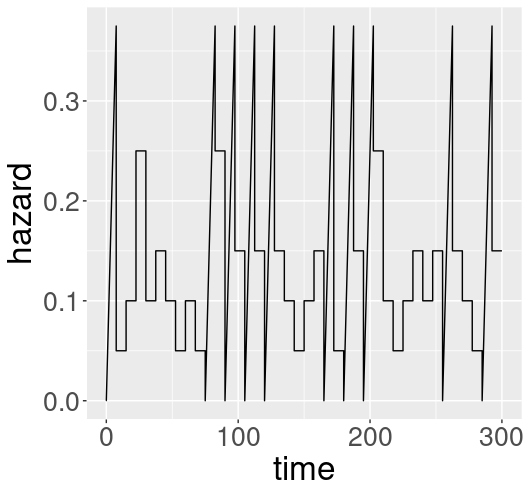
\includegraphics[width=0.55\textwidth,height=2.5in]{true_base.png}
\caption{True Baseline Hazard in the example in \ref{subsubsec:sim2}.}
\label{fig:truebase}
\end{figure}

\begin{figure}[ht]
\centering
\subfigure[Posterior effect of \texttt{tpi}]{
  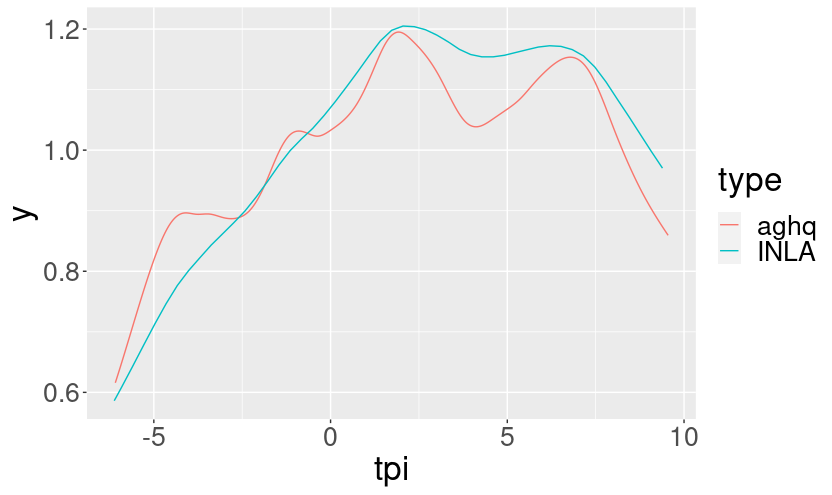
\includegraphics[width=0.45\textwidth,height=2.5in]{leukSmooth.png}
}
\subfigure[Posterior distribution of $\sigma$]{
  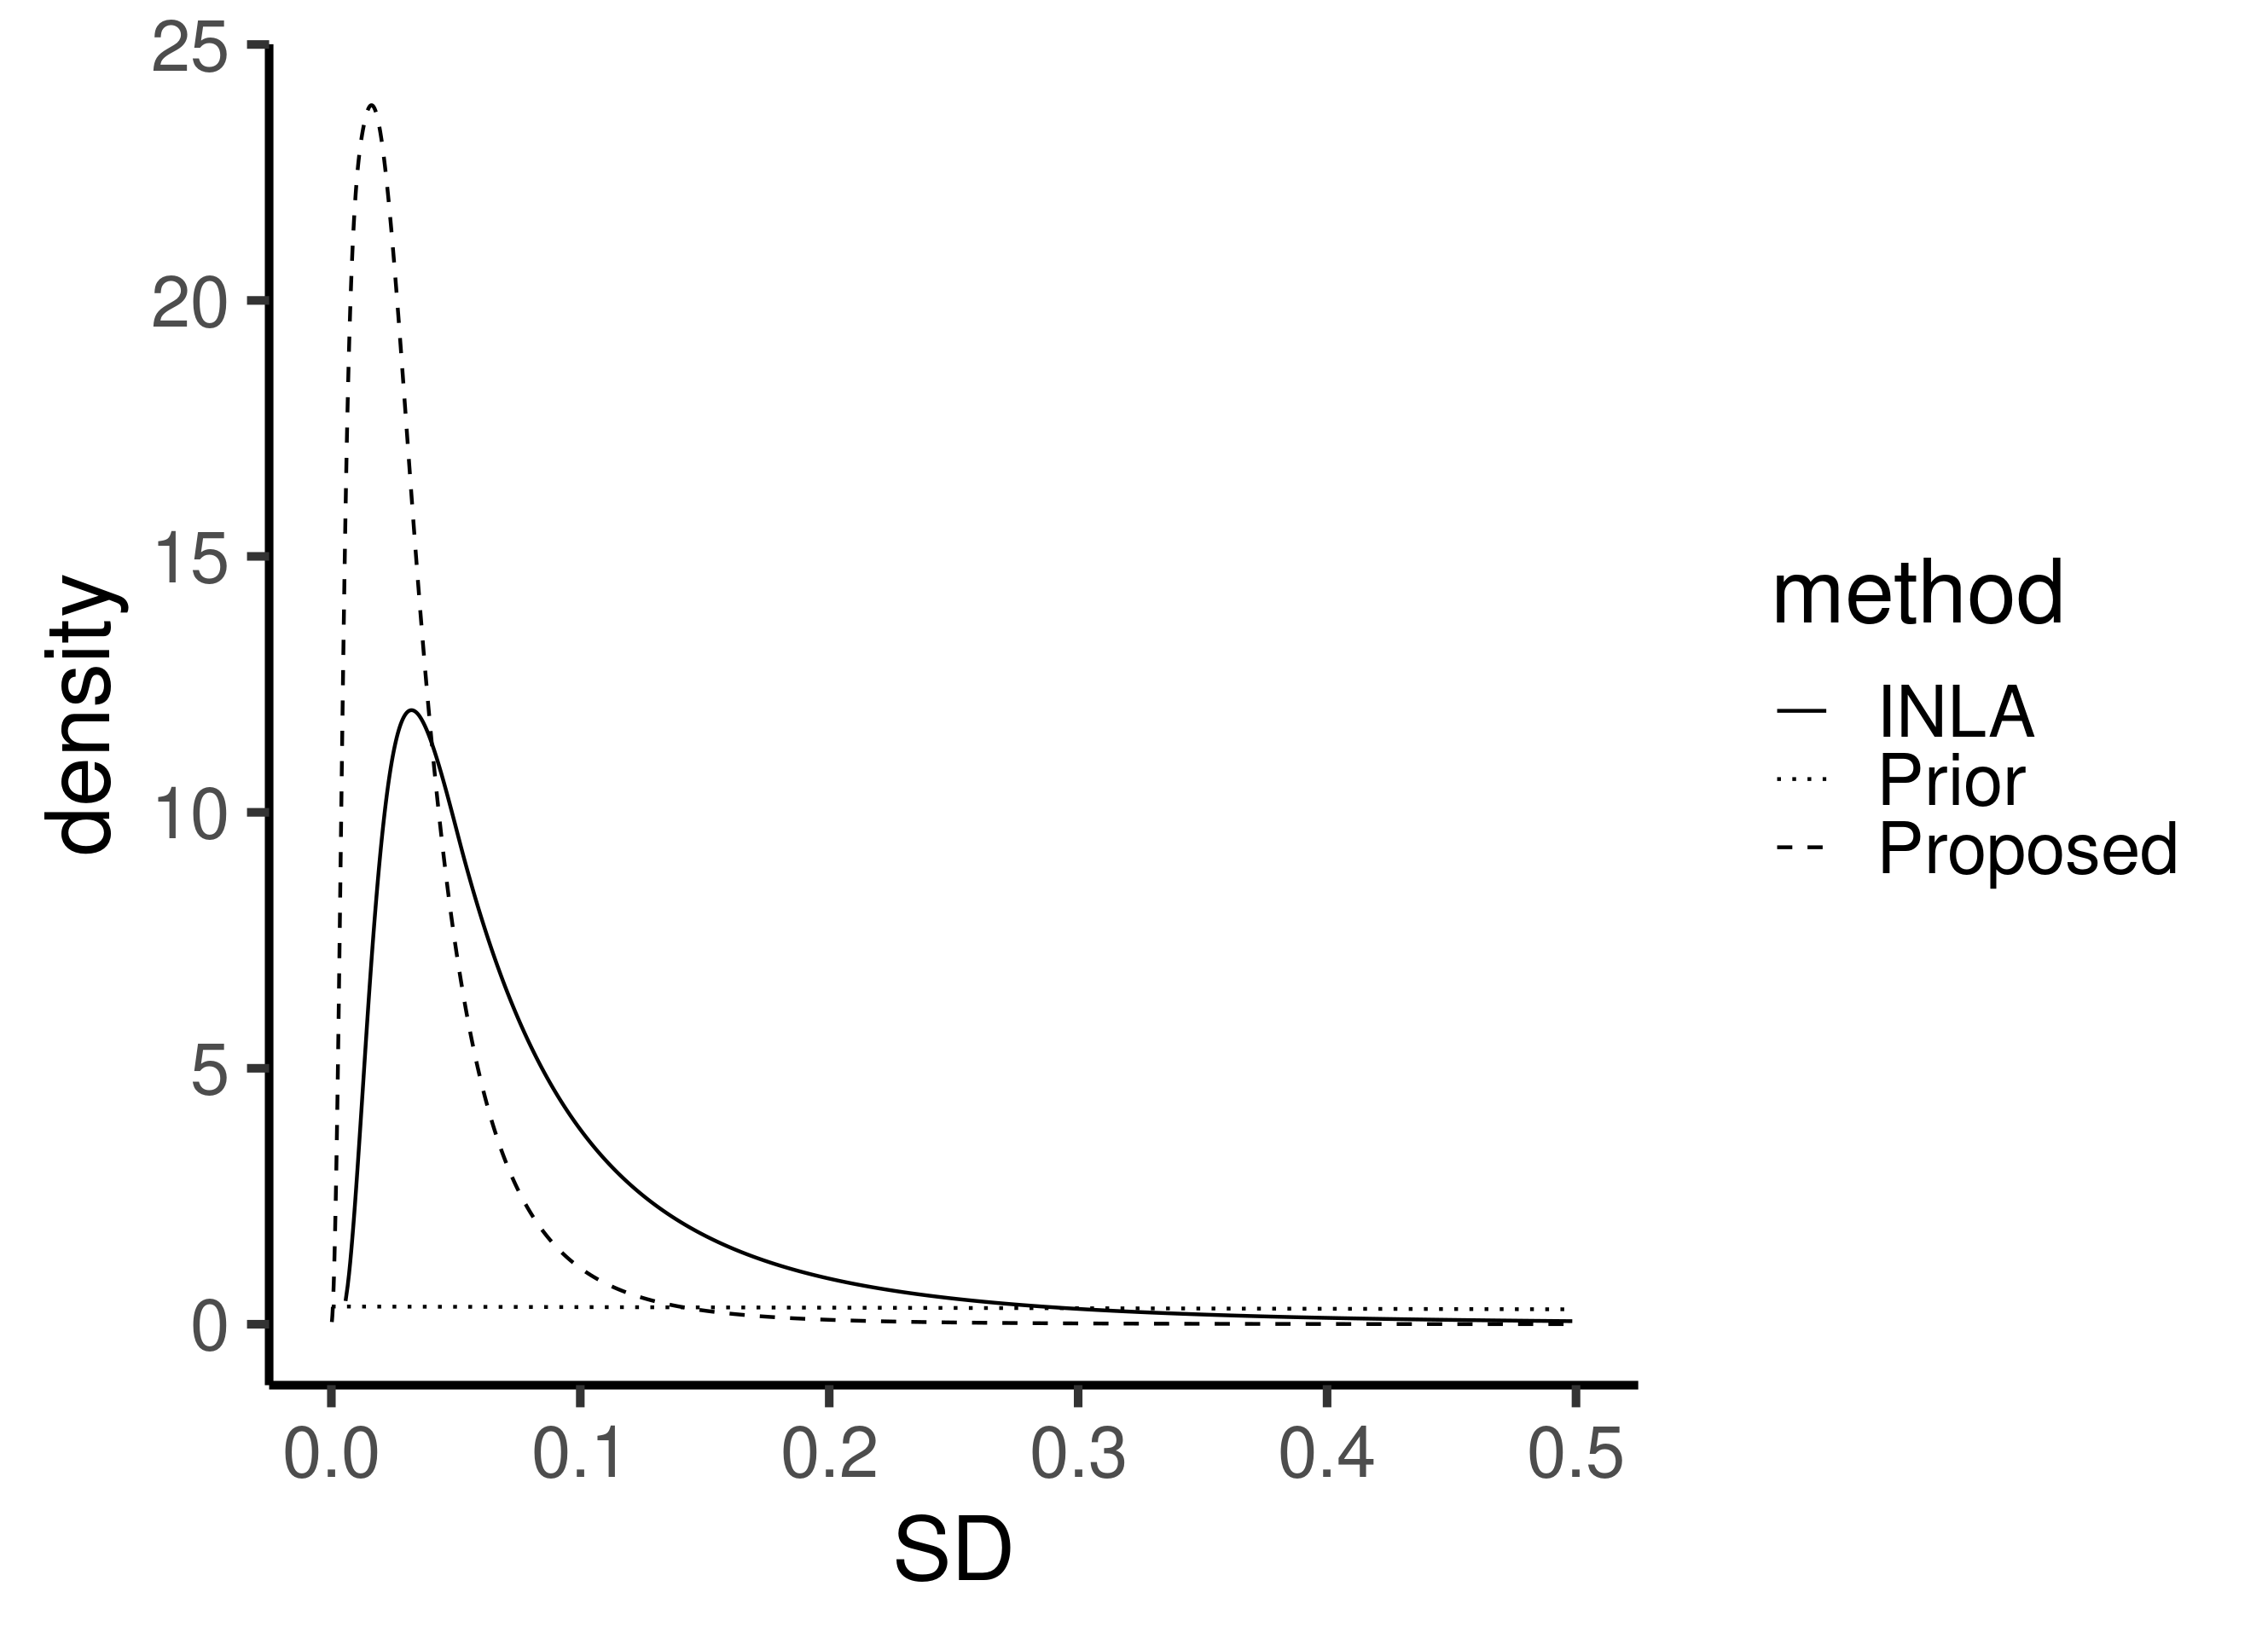
\includegraphics[width=0.45\textwidth,height=2.5in]{leukHyper.png}
}
\subfigure[Posterior cumulative distributions of $\sigma$]{
	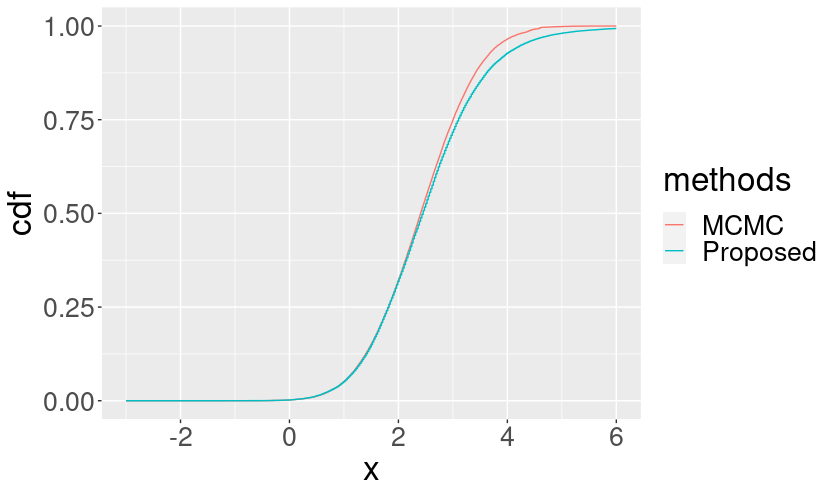
\includegraphics[width=0.55\textwidth,height=2.5in]{leuk_KS.png}
}
\caption{Results for the Leukaemia data in section \ref{subsec:leuk}. (a): (Exponentiated) posterior mean for the semi-parametric tpi effect using our proposed method(red) and INLA(blue) (b): Posterior distribution for $\sigma$ obtained using MCMC(blue histogram), and using the proposed method(black line). (c): Posterior cumulative distribution for $\sigma$ obtained using MCMC(red) and using the proposed method(blue)}
\label{fig:leuk}
\end{figure}



\begin{table}
\begin{center}
\scalebox{0.99}{
\begin{tabular}
{|p{3cm}|
p{1cm}|p{1cm}p{1cm}|p{1cm}p{1cm}|}
\hline
\cline{1-6}
      \multicolumn{1}{l}{} &
      \multicolumn{1}{l}{} &
      \multicolumn{2}{c}{Proposed} &
      \multicolumn{2}{c}{INLA}\\
      Variables/Reference & Levels & {Mean} & {SD} & {Mean} & {SD} \\
 \hline
 Age & & 0.00467 & 0.0149 & 0.00235 & 0.0130 \\
 Sex/Male & Female & -1.65  & 0.463  & -1.64 & 0.385 \\
 Disease Type/Other & GN & 0.178 & 0.532 &  0.111 & 0.474 \\
  & AN & 0.420 & 0.528 & 0.519 & 0.467  \\
  & PKD & -1.15 & 0.817  & -1.06 & 0.708 \\
\hline
\end{tabular}
}
\end{center}
\caption{Estimated means and standard deviations of linear effects by proposed method and INLA's full likelihood method for the kidney data in section \ref{subsec:kidney}. }
\label{table:KidneyFixed1}
\end{table}





\begin{table}
\begin{center}
\scalebox{0.99}{
\begin{tabular}
{|p{3cm}|
p{1cm}|p{1cm}p{1cm}|p{1cm}p{1cm}|}
\hline
\cline{1-6}
      \multicolumn{1}{l}{} &
      \multicolumn{1}{l}{} &
      \multicolumn{2}{c}{Proposed} &
      \multicolumn{2}{c}{MCMC}\\
      Variables/Reference & Levels & {Mean} & {SD} & {Mean} & {SD} \\
 \hline
 Age & & 0.00467 & 0.0149 & 0.00516 & 0.0158 \\
 Sex/Male & Female & -1.65  & 0.463  & -1.72 & 0.507 \\
 Disease Type/Other & GN & 0.178 & 0.532 &  0.172 & 0.576 \\
  & AN & 0.420 & 0.528 & 0.415 & 0.573  \\
  & PKD & -1.15 & 0.817  & -1.26 & 0.859 \\
\hline
\end{tabular}
}
\end{center}
\caption{Estimated means and standard deviations of linear effects by proposed method and MCMC method for the kidney data in section \ref{subsec:kidney}. }
\label{table:KidneyFixed2}
\end{table}




\begin{figure}[ht]
\centering
\subfigure[Posterior distributions of $\sigma$]{
  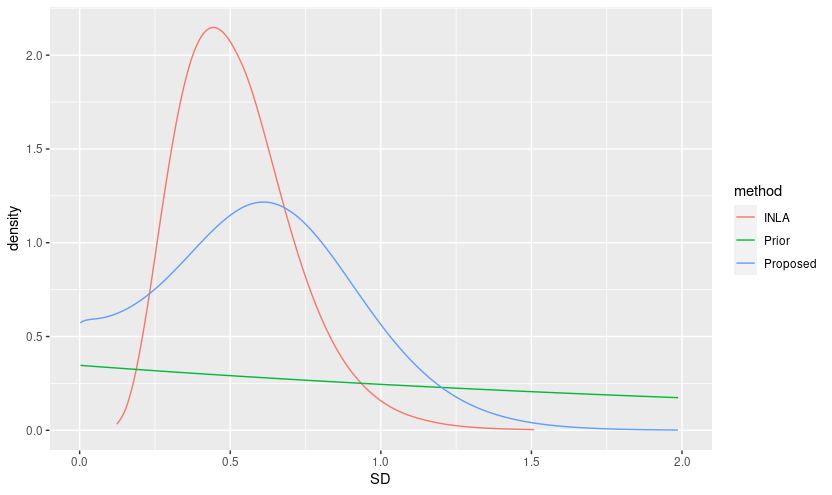
\includegraphics[width=0.45\textwidth,height=2.5in]{kidneyHyper.png}
}
\subfigure[Posterior distributions of $\sigma$]{
  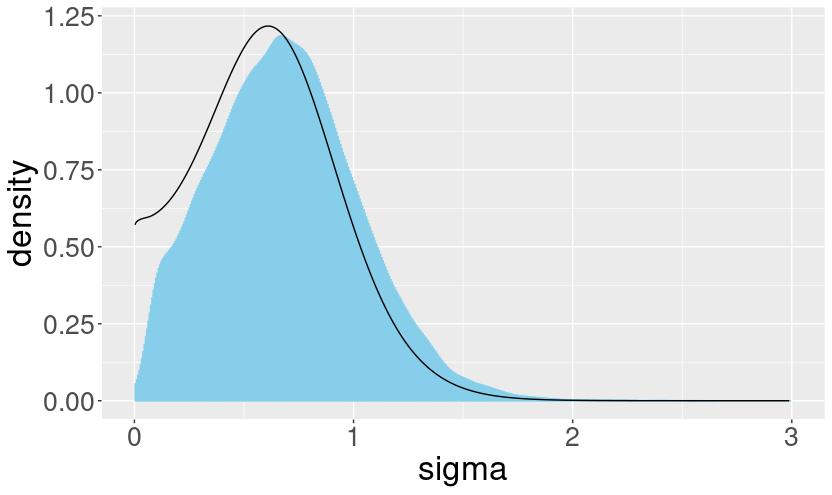
\includegraphics[width=0.45\textwidth,height=2.5in]{kidneyHyper2.png}
}
\subfigure[Posterior cumulative distributions of $\sigma$]{
	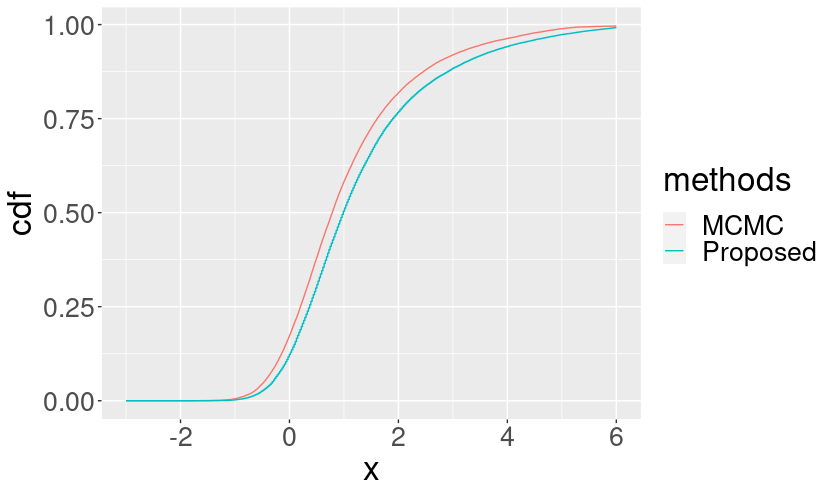
\includegraphics[width=0.55\textwidth,height=2.5in]{kidneyKS.png}
}
\caption{Results for the kidney data in section \ref{subsec:kidney}. (a): Prior(green) and posterior distributions for $\sigma$ using our proposed method(blue) and INLA(red) (b): Posterior distribution for $\sigma$ obtained using MCMC(blue histogram), and using the proposed method(black line). (c): Posterior cumulative distribution for $\sigma$ obtained using MCMC(red) and using the proposed method(blue)}
\label{fig:kidneyHyper}
\end{figure}





\end{document}

